\documentclass{vldb}
\usepackage{graphicx}
\usepackage{balance}  % for  \balance command ON LAST PAGE  (only there!)

% ****************** sungsoo's packages ****************************************
\usepackage{times}
%                              My Commands
\newcommand{\bi}{\begin{itemize}}
\newcommand{\ei}{\end{itemize}}
\newcommand{\be}{\begin{enumerate}}
\newcommand{\ee}{\end{enumerate}}
\newcommand{\ii}{\item}
\newtheorem{Def}{Definition}
\newtheorem{Lem}{Lemma}
\usepackage{algorithm}
\usepackage{algorithmicx}
\usepackage{algpseudocode}

%\usepackage[]{algorithm2e}

\usepackage{graphicx}
\graphicspath{%
        {converted_graphics/}
        {./images/}
}
\usepackage{hyperref}
\usepackage{listings}
\usepackage{longtable}

% ****************** the following is needed for syntax highlighting
\usepackage{color}

\definecolor{dkgreen}{rgb}{0,0.6,0}
\definecolor{gray}{rgb}{0.5,0.5,0.5}
\definecolor{mauve}{rgb}{0.58,0,0.82}

\lstset{ %
  language=Java,                  % the language of the code
  basicstyle=\scriptsize,       % the size of the fonts that are used for the code
  numbers=left,                   % where to put the line-numbers
  numberstyle=\tiny\color{gray},  % the style that is used for the line-numbers
  stepnumber=1,                   % the step between two line-numbers. If it's 1, each line 
                                  % will be numbered
  numbersep=3.8pt,                  % how far the line-numbers are from the code
  backgroundcolor=\color{white},  % choose the background color. You must add \usepackage{color}
  showspaces=false,               % show spaces adding particular underscores
  showstringspaces=false,         % underline spaces within strings
  showtabs=false,                 % show tabs within strings adding particular underscores
  frame=false,                   % adds a frame around the code
  rulecolor=\color{black},        % if not set, the frame-color may be changed on line-breaks within not-black text (e.g. commens (green here))
  tabsize=2,                      % sets default tabsize to 2 spaces
  captionpos=b,                   % sets the caption-position to bottom
  breaklines=true,                % sets automatic line breaking
  breakatwhitespace=false,        % sets if automatic breaks should only happen at whitespace
  title=\lstname,                 % show the filename of files included with \lstinputlisting;
                                  % also try caption instead of title
  keywordstyle=\color{blue},          % keyword style
  commentstyle=\color{dkgreen},       % comment style
  stringstyle=\color{mauve},         % string literal style
  escapeinside={\%*}{*)},            % if you want to add a comment within your code
  morekeywords={*,...}               % if you want to add more keywords to the set
}
% ****************** end of sungsoo's packages ****************************************


\begin{document}

% ****************** TITLE ****************************************

%\title{A Sample {\ttlit Proceedings of the VLDB Endowment} Paper in LaTeX
%Format\titlenote{for use with vldb.cls}}

\title{Scalable Stream Data Processing for the Performance Monitoring of Critical Equipments in the Offshore Plants}

\numberofauthors{1} %  in this sample file, there are a *total*
% of EIGHT authors. SIX appear on the 'first-page' (for formatting
% reasons) and the remaining two appear in the \additionalauthors section.

\author{
% 1st. author
\alignauthor
Sung-Soo Kim\\ %\titlenote{Dr.~Trovato insisted his name be first.}\\
       \affaddr{Data Management Research Section}\\
       \affaddr{Electronics and Telecommunications Research Institute}\\
       \affaddr{128 Gajeong-ro, Yuseong-gu}\\
       \affaddr{Daejeon, South Korea}\\
       \email{\normalsize \it sungsoo@etri.re.kr}
}

\maketitle

% !TEX root = demo.tex
\begin{abstract}
%The prevalence of dirty data presents a fundamental obstacle to modern data-driven applications.
Analysts report spending upwards of 80\% of their time on problems in data cleaning.
The data cleaning process is inherently iterative, with evolving cleaning workflows that 
start with basic exploratory data analysis on small samples of dirty data, then refine analysis with 
more sophisticated/expensive cleaning operators (e.g., crowdsourcing), and finally apply the insights to a full dataset.
While an analyst often knows at a logical level what operations need to be done, they often have 
to manage a large search space of physical operators and parameters.
We present \sys, a system designed to support the iterative development and optimization of data cleaning workflows, especially ones that utilize the crowd.
\sys separates logical operations from physical implementations, and driven by analyst feedback, suggests optimizations and/or replacements to the analyst's choice of physical implementation.
We highlight research challenges in sampling, in-flight operator replacement, and crowdsourcing. 
We overview the system architecture and these techniques, 
then provide a demonstration designed to showcase how \sys can improve iterative data analysis
and cleaning. 
The code is available at: \url{http://www.sampleclean.org}.
\end{abstract}



% !TEX root = demo.tex
\section{Introduction}\label{sec:intro}

\begin{figure}[t]
\centering
\vspace{-0.5cm}
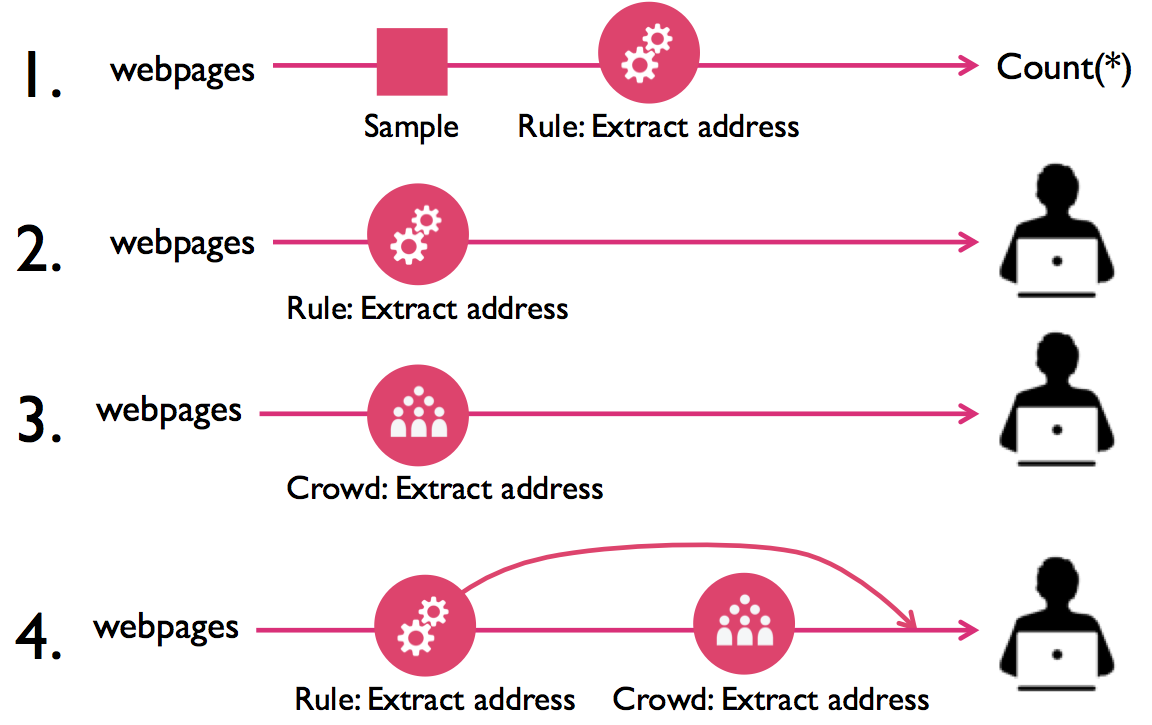
\includegraphics[width = .4\textwidth]{figs/lifecycle.png}
\vspace{-0.4cm}
\caption{Example iterations on the design of the portion of a cleaning plan that extracts restaurant addresses from their unstructured webpages.  
1) An exploratory plan that uses a sample to evaluate a simple address extraction method.
2) A plan that applies the method to the entire dataset. The quality is unsatisfactory. 
3) An alternate plan that uses manual crowd extraction. The quality is now high, but the crowd-based extractor is slow. 
4) A hybrid plan that sends only difficult webpages to the crowd, maximizing accuracy without sacrificing latency.}
\label{fig:ex-plan}
\vspace{-0.3cm}
\end{figure}
% why feedback loops exist/are important (cite Joe’s shit in the past 3 years, blinkdb, etc.). highlight domain specificity. Large variety of data cleaning tasks

%
% General comment that data cleaning is important:
%
The ease of acquiring and merging many large-scale data sources has led to a prevalence of dirty data.
Unfortunately, blindly using results that are derived from dirty data can lead to hidden yet significant errors in modern data-driven applications, so data must be cleaned before it is used.
But because data cleaning is often specific to the domain, dataset, and eventual analysis, analysts report spending upwards of 80\% of their time on problems in data cleaning~\cite{kandel2012}.
The analyst is faced with a breadth of possible errors that are manifest in the data and a variety of options to resolve them.
She must go through the cleaning process via trial and error, deciding for each of her data sources what to extract, how to clean it, and whether that cleaning will significantly change results.

Data cleaning is inherently iterative and Figure~\ref{fig:ex-plan} shows a common progression for the development of a data cleaning plan, in this case the extraction of a restaurant's address from its unstructured webpage.
While this operation can easily be represented at a \textit{logical} level by its input and output schema, there is a huge space of possible \textit{physical} implementations of the logical operators. 
For example, extraction could depend on manually specified rules (\textit{rule-based}), use models trained on previously extracted ground truth records (\textit{learning-based}), ask crowd workers to extract the desired data fields (\textit{crowd-based}), or some combination of the three (e.g., active learning, which uses crowd workers to provide labels for a learning-based approach).
Even after selecting (say) a crowd-based operator, many parameters might influence the quality of the output data or the speed and cost of cleaning: the number of crowd workers who vote on the extraction for a given webpage, the amount each worker is paid, etc.
A priori, a data analyst has little intuition for what physical plan will be optimal in this large space.

Note that in the evolution of the data cleaning plan in Figure~\ref{fig:ex-plan}, our data analyst needed to make many decisions manually about the choice of physical operators by reasoning about their latency, accuracy, and cost. 
Making the wrong decision, for example using the crowd when it only marginally improves accuracy, can be very costly.
A general, scalable, and interactive system that supports rapid iteration on candidate plans would greatly aid this process.

%The prevalance of data cleaning systems in both the research and industrial communities --
%Corleone does blah, XXX addresses blah. Nadeef does blah -- speak to the importance of a
%data cleaning framework as part of the modern big data ecosystems. \ewu{include open access of data in argument?} \jn{We also need to take a look at data cleaning systems in industry. }


% why existing systems suck aka related work
% 1. have slow feedback loops (dataset-dependence, …)
% 2. solve very specific data-cleaning tasks
%Since the beginning of data management, systems have been explored by both the research and industrial communities to improve data cleaning efficiency and quality.
Existing systems seldom address the end-to-end iterative data cleaning process described above.
Extract-transform-load (ETL) systems~\cite{informatica,talend,apachefalcon} require developers to manually write data cleaning rules and execute them as long batch jobs, 
and constraint-driven tools allow analysts to define ``data quality rules" and automatically propose corrections to maximally satisfy these rules \cite{DBLP:conf/sigmod/DallachiesaEEEIOT13}.
Unfortunately, neither provide the opportunity for iteration or user feedback, inhibiting the user's ability to rapidly prototype different data cleaning solutions.
Projects such as Wrangler~\cite{wrangler,trifacta} and OpenRefine~\cite{openrefine} support iteration with spreadsheet-style interfaces that enable the user to compose data cleaning sequences by directly manipulating a sample of the data and applying these sequences to the full dataset.
However, they are limited to specific cleaning tasks such as simple text transformations, do not support crowd-based processing at scale, and cannot incorporate user feedback to optimize the physical implementation of the data cleaning sequences.
Crowd-based~\cite{gokhale2014corleone,stonebraker2013data} systems have been proposed to relieve the data analyst of the burden of rule specification or manual cleaning, but are usually specific to a single cleaning task (e.g.,~\cite{gokhale2014corleone,park2014crowdfill,eracer,chen2014integrating}), preventing end-to-end optimization of the entire cleaning plan.
These existing limitations suggest the need for a system that is general enough to adapt to a wide range of data cleaning applications, scales to large datasets, and natively supports fast-feedback interactions to enable rapid data cleaning iteration.

In this paper, we introduce \sys, a system designed to support the iterative development and optimization of data cleaning plans end to end.
\sys allows users to specify declarative data cleaning plans composed of rule-based, learning-based, or crowd-based operators, then iterate rapidly on plans with cost-aware recommendations for improving the accuracy or latency of a plan.
The effects of a plan can be viewed early using sampling and approximate query processing techniques~\cite{wang1999sample}.

Supporting these capabilities requires a combination of careful engineering 
as well as tackling several research challenges:

\squishlist
\item \textbf{Sampling}: We provide sampling as a first-class logical operator for data cleaning plans that tolerate approximation, and use it to speed up iteration on early-stage plans.

\item \textbf{Recommendation}: We recommend cost-aware changes to in-flight cleaning plans that allow users to trade off accuracy and latency, and provide efficient mechanisms for implementing recommended changes without re-executing the plan on already cleaned tuples.

\item \textbf{Crowd Latency}: We leverage techniques for straggler mitigation~\cite{venkataraman2014power} and model crowd worker speed and accuracy to reduce the (often rate-limiting) latency of crowd data cleaning, consistently retrieving results in seconds rather than hours.
\squishend

In our demonstration, we will run an entity resolution plan on two restaurant datasets, and
show how \sys can be used to 1) specify, modify, and execute a data cleaning plan,
2) quickly clean a sample to characterize how a plan is performing, and
3) observe the same cleaning plans running on multiple datasets.
Users can execute plans over a live crowd that uses the audience as workers, or a simulated crowd
that uses pre-collected crowd responses. The dashboard (Figure~\ref{screenshot}) also provides a live inspection
interface to view the status of the cleaning plan as it executes.

\vspace{-0.2cm}
%Our contributions/requirements
%different ways to tighten the feedback loop:
%end-to-end latency/cost (operator optimization)
%looking versus touching
%Adding introspection (more points of observation)
%hot-swapping (more points of changing plans)
%We have built an end-to-end data cleaning framework with these requirements in mind. (... things we do …) (... engineering contributions …).
%In this demonstration, we highlight the benefits of improving feedback loops for data cleaning using X datasets by optimizing a data cleaning pipeline for one data set/cleaning task, then quickly fitting the pipeline to another dataset.


\if{0}

\jn{Honestly, I didn't quite buy declarativity of the system. In my opinion, data cleaning is so domain specific. It's hard to make it declarative. For a given domain, people may need to write their own data cleaning system. There is a lack of a data cleaning framework that they can build based on. This motivates us to develop such framework. 


We analyze a large variety of domain specific data cleaning systems, and identify several key components: declarative data cleaning operators (e.g., similarity joins), active learning, and crowd/expert sourcing platforms that they require. In our framework, we abstract these components, and implement them in a general way. 

We mainly address two challenges: extensibility and scalability. For the former one, we came up with a nice data-cleaning pipeline API, which people can easily use to compose their own data cleaning tasks. For the latter one, we address it in two aspects: Sampling + Asynchrony.}

\ewu{That's fair, will need to address why a framework is necessary and what benefits it provides.  I think a framework is the correct pitch, hard to sell a set of operators.  Are the above challenges -- extensibility and scalability -- actually difficult?  Worried it's straightforward application of existing techniques.}



In contrast, our work is based on the observation that the majority of data cleaning workflows
can be decomposed into a small set of logical operations (in addition to traditional database operators):
filter based on constraints, extract new fields from existing data, and a similarity join to match
similar or duplicate records. \ewu{quickly validate why this observation holds.} \jn{Yes! I also found that Sec 2.3 has more operators than you describe here.}  
By designing a system around these core operators, we can provide a vast library of physical  
data cleaning operators that span the range of algorithmic, machine learning, and human computation-based
implementations that are necessary practical data cleaning pipelines.   \ewu{Describe live inspection as 
a core feature or is it too easy?}

Designing such a system requires tackling several design challenges:

\begin{enumerate}
\item Speed
\item Quality
\item API Design/extensibilty
\end{enumerate}



We have implemented an initial version of \sys on top of the AMPLab Spark stack, which provides us 
with access to its advanced distributed processing and machine learning features.  Our goal for the current
version is to implement the core mechanisms for declarative specification of the
data cleaning pipeline, solidify the API design, and incle support for, and implementations of,
multiple classes of physical data cleaning operators.


\fi



\if{0}

Cleaning, pre-processing, and formatting data is a required first step in any data analytics pipeline.
However, despite this importance, large-scale data analytics platforms such as Spark or Hadoop lack integrated data cleaning frameworks.
There are a few challenges in building a general purpose data cleaning framework: (1) data cleaning is often
domain specific and requires specialized software targeted at one or a handful of data sources \cite{wang1999sample}, (2) data cleaning is often 
expensive as it increasingly involves human effort via crowdsourcing or experts \cite{DBLP:conf/sigmod/GokhaleDDNRSZ14}, and (3) learning how to clean dirty data from examples
is often hard without a greatly restricted set of operators \cite{DBLP:conf/uist/GuoKHH11}.

We address this problem in \projx by designing a Spark library of composable and scalable data cleaning primitives.
\projx abstracts the logical data cleaning operators: Extraction, Similarity Join, Filtering, from the physical implementation i.e, Rule, Crowd, or Machine Learning.
We interface these primitives through a DSL with which a user can build data cleaning operators that suit their needs.
\projx provides transparent optimizations for each of the components and their composition.
In this demonstration proposal, we present \projx and highlight some of its key features.
While there are many existing systems that do one aspect of data cleaning and transformation (e.g Entity Resolution or Extraction), 
many real world data cleaning tasks have multiple types of errors.
Composing disparate systems can lead to complex code and inefficiencies at scale.
With \projx, we hope to design a set of optimized composable primitives that span a large space of data cleaning tasks.

The first key feature of \projx is that it provides optimized distributed implementations 
of the physical data cleaning operators.
For example, a key step in many deduplication algorithms is a Similarity Join which finds all pairs of records that are within some similarity threshold.
A naive implementation of a Similarity Join would apply a similarity function to all pairs of records.
However, in \projx, we provide optimized implementations of certain common similarity functions (e.g Jaccard, Edit Distance, etc.) that allow for 
a combined broadcast join and prefix filtering which intelligently skips pairs of records using a broadcasted inverted index.

Another feature of \projx is managing the latency and the scale problems of crowd-based data cleaning. 
Crowdsourcing is increasingly prevalent in data cleaning, and \projx provides physical crowd-based implementations
of the logical operators.
However, crowds work at a different latency and scale point in comparison to distributed analytics platforms.
To address the latency problem, we build asychrony into the system.
The user can query intermediate results at any time as crowd responses stream in.
To address the scale issue, \projx provides sampling primitives.
The glue that ties all of the crowd components together is a Machine Learning technique called Active Learning.
As we collect more and more crowd responses, we learn a model that predicts these responses to apply it on the uncleaned data.
Active Learning selects the most informative questions to ask the crowd.

Finally, \projx provides an approximate query processing (AQP) framework.
With slow asynchronous data cleaning algorithms as in crowdsourcing, we need 
to define clear semantics for the intermediate results.
Our AQP framework uses the algorithms proposed in \cite{wang1999sample}, to estimate and bound early results.
It is also common for data scientists to prototype expensive data cleaning pipelines on samples and AQP allows quick evaluation of
aggregate query results on a cleaned sample.

\subsection{Demonstration Scenario}
\reminder{TODO}

\fi




\if{0}
Consider for example, the ability to rapidly understand the types of errors that are present, as well as prevalance of 
these errors is cruicial.



Before an organization can use a new dataset as part of their analysis pipeline
(e.g., to build complex learning models or answer analyst queries)
the errors in the dataset need to be removed in order to ensure accurate conclusions.  

Modern data-driven organizations rely on the ability to ingest and generate large data sets from 
disparate sources, and combine the data together to build complex models or answer analytical questions.  
For example, a restaurant review website may collect restaurant listings by scraping data from webpages or purchasing them from external sources, and
restaurant visitation information for sources such as OpenTable or FourSquare, and aggregate the data to
model user eating habits.  
The set of cleaning tasks necessary for each of these data sources is highly domain and application specific,
and oftentimes the developer is concurrently trying to clean the data source as well as understand its properties.


Oftentimes, these data sources have data quality issues that require a complex data cleaning pipeline -- 
e.g., data extraction, re-formatting, identification and fixes of missing or incorrect values,
and removal of redundant information -- before the data is useable by downstream processes.
Data sources are often domain specific and new for the data analyst, 
As datasets continue to grow, and organizations make use of mure and more datasets, the ability to
rapidly clean the data is more important.  
\fi


\section{Related Work}

\section{Body}

\subsection{Problem Definition}

\subsection{Approach}

\subsection{Architecture}

\section{Results}

\subsection{Evaluation and Analysis}


\vspace{-.5em}
\section{Conclusion and Future Work}\label{sec:con}
In this paper, we explore using sampling, integrated with data cleaning, to improve answer quality. We propose \saqpplus, a novel framework which only requires users to clean a sample of data, and utilizes the cleaned sample to obtain unbiased query results with confidence intervals.
We identify three types of data errors (i.e., value error, condition error and duplication error) that may affect query results, and develop \biascorrected and \sampleclean to estimate query results for the data with these errors.
Our analysis and experiments suggest that \saqpplus, which returns the better result between \biascorrected and \sampleclean, is robust to different magnitudes and rates of data errors, and consistently reports good estimate results.
%Moreover, \saqpplus can optimally satisfy user-specified cleaning-cost or result-quality constraints.
Our experiments on both real and synthetic data sets indicate that \saqpplus only needs to clean a small sample of the data to achieve accurate results, and furthermore the size of this sample is independent of the size of the dataset.
In particular, \sampleclean, which processes queries only on the cleaned sample, not only makes the query processing more scalable, but surprisingly may provide higher quality results than an aggregation of the entire dirty data (\alldirty).

To the best of our knowledge, this is the first work to marry data cleaning with sampling-based query processing.
%But, it is merely the tip of the iceberg.
There are many research directions for future exploration. 

\vspace{.25em}
{\noindent \bf Constrained Queries:} Now that we have quantified a tradeoff between cleaning costs and result quality, we can explore query results where users can specify a cost or quality constraint. For example, users may want to know that given a cleaning budget, what is the best result quality they can achieve? Or, given a quality constraint, how many samples they need clean to meet the constraint? 
In these constrained queries, we aim to answer with an optimal cost or most accurate result to meet the constraints.

\vspace{.25em}
{\noindent \bf Uncertain Cleaning Results:}  Our framework can return unbiased query results with respect to AllClean for a variety of different data cleaning approaches.
We are also interested in how we can incorporate uncertain or probabilistic cleaning processes into this framework.
For example, given a dirty record, could the data cleaning module specify a set of ranges for each attribute? 
We are interested in what guarantees, if any, we can achieve in such settings.

\vspace{.25em}
{\noindent \bf Complex SQL Queries:} Another important avenue of future work is to extend our framework to support more complex SQL queries such as join and nested SQL queries. There are some straightforward methods to implement these queries. For example, we can materialize the join result as a single table, and then apply our framework to the materialized table. But this could be very costly for large datasets, thus we need to explore more efficient implementations.
For a larger set of queries, it may not be possible to estimate their results with the CLT.
Thus, exploring empirical estimation approaches (such as bootstrapping) to our framework is another interesting future direction.

\vspace{.25em}
{\noindent \bf Sample Maintenance:} Finally, in real applications users may create multiple samples from the data.
Maintaining these samples for data updates is also very challenging and needs to be investigated.


\vspace{1.5em}

\fussy
{\noindent  \bf Acknowledgements.} {\small  The authors would like to thank Sameer Agarwal, Bill Zhao, and the SIGMOD reviewers for their insightful feedback. This research is supported in part by NSF CISE Expeditions Award CCF-1139158, LBNL Award 7076018, DARPA XData Award FA8750-12-2-0331, the European Research Council under the FP7, ERC MoDaS, agreement 291071, and by the Israel Ministry of Science, and gifts from Amazon Web Services, Google, SAP, The Thomas and Stacey Siebel Foundation, Apple, Inc., Cisco, Cloudera, EMC, Ericsson, Facebook, GameOnTalis, Guavus, Hortonworks, Huawei, Intel, Microsoft, NetApp, Pivotal, Samsung, Splunk, Virdata, VMware, WANdisco and Yahoo!.
}
\sloppy





\bibliographystyle{abbrv}
\bibliography{references}

\end{document}
